\documentclass{article}
% Generated by code/run_all.py; do not edit.
\newcommand{\PageMargin}{0.9in}
\newcommand{\LineSpread}{1.08}
\newcommand{\PlotWidth}{0.98}
\newcommand{\AuthorEmail}{jpbald93@gmail.com}
\newcommand{\AIAstra}{GPT-6 Astra}
\newcommand{\AIOpus}{Claude Opus 5.5 (Anthropic)}
\newcommand{\AIPlatform}{the Genspark platform}
\newcommand{\RepoURL}{\url{https://github.com/jpbald93/trotter-depth-tutorial}}
\newcommand{\Nqubits}{6}
\newcommand{\HilbertDim}{64}
\newcommand{\Jval}{0.7}
\newcommand{\Hval}{1.05}
\newcommand{\Tval}{0.8}
\newcommand{\ThetaVal}{0.9}
\newcommand{\PhiVal}{0.0}
\newcommand{\Nmax}{64}
\newcommand{\Ncal}{16}
\newcommand{\TailStart}{32}
\newcommand{\Pcal}{1\times 10^{-7}}
\newcommand{\Reps}{400}
\newcommand{\Seed}{20260924}
\newcommand{\DeltaVal}{0.05}
\newcommand{\LowerPercentile}{10}
\newcommand{\UpperPercentile}{90}
\newcommand{\ExactVal}{0.53013405}
\newcommand{\CommVal}{2.100}
\newcommand{\Tolerance}{1\times 10^{-10}}
\newcommand{\CleanOne}{0.00639}
\newcommand{\CleanTwo}{1.29\times 10^{-5}}
\newcommand{\AOne}{0.41}
\newcommand{\ATwo}{0.0527}
\newcommand{\COne}{1.87}
\newcommand{\CTwo}{2.69}
\newcommand{\GOne}{11}
\newcommand{\GTwo}{17}
\newcommand{\Comparisons}{63}
\newcommand{\BlockComm}{10.3}
\newcommand{\ABound}{6.57}
\newcommand{\NoiseBound}{22}
\newcommand{\ALooseness}{16}
\newcommand{\CLooseness}{11.8}
\newcommand{\CancelMatches}{3}
\newcommand{\CancelCases}{3}
\newcommand{\LateHighCases}{4}
\newcommand{\HighCases}{6}
\newcommand{\EarlyHighDepth}{41}
\newcommand{\EarlyHighOpt}{46}
\newcommand{\BoundaryDepth}{2}
\newcommand{\BoundaryBias}{-0.0807}
\newcommand{\PLow}{0.0001}
\newcommand{\PMid}{0.0005}
\newcommand{\PHigh}{0.002}
\newcommand{\ShotsLow}{1\times 10^{4}}
\newcommand{\ShotsMid}{1\times 10^{6}}
\newcommand{\ShotsHigh}{1\times 10^{10}}
\newcommand{\TauLow}{0.056}
\newcommand{\TauMid}{0.0056}
\newcommand{\TauHigh}{5.6\times 10^{-5}}

\usepackage[margin=\PageMargin]{geometry}
\usepackage{amsmath,amssymb,amsthm,mathtools,booktabs,graphicx}
\usepackage{lmodern}
\usepackage[colorlinks=true,linkcolor=blue,citecolor=blue,urlcolor=blue]{hyperref}
\linespread{\LineSpread}
\newtheorem{theorem}{Theorem}
\newtheorem{proposition}{Proposition}
\newtheorem{assumption}{Model assumption}
\newcommand{\Tr}{\operatorname{Tr}}
\DeclarePairedDelimiter{\norm}{\lVert}{\rVert}
\DeclarePairedDelimiter{\abs}{\lvert}{\rvert}
\title{Noise-limited Trotter depth and a shot-noise stopping rule:\\a reproducible tutorial}
\author{Josh Bald\\Independent researcher, Ontario, Canada\\\texttt{\AuthorEmail}}
\date{}
\begin{document}
\maketitle
\begin{abstract}
Increasing the number of product-formula steps reduces discretization error but adds noisy gates. This tutorial derives the minimum of an algebraic error surrogate, distinguishes a rigorous upper bound from an observable-specific fit, and explains how finite-shot uncertainty limits depth selection. Dense density-matrix simulations of a small spin chain illustrate both useful predictions and failures caused by signed-error cancellation. A finite-shot stopping rule is explicitly a heuristic, not a certificate of optimality. This paper claims no novelty beyond clear presentation and reproducible worked examples. All experimental numerical quantities, tables, figures, and bibliographic metadata are generated by the accompanying code; the manuscript includes symbolic and numerical checks.
\end{abstract}

\section{Purpose, prior work, and the three kinds of statement}
Product formulas approximate an evolution generated by a sum of noncommuting Hamiltonian terms by a sequence of implementable evolutions. Lloyd's universal-simulation construction is foundational context \cite{lloyd}; Suzuki's higher-order decompositions provide the structural background for symmetric formulas \cite{suzuki}. Modern commutator bounds explain why error constants depend on more than just the norm of the entire Hamiltonian \cite{childs}. Faulty control changes the depth-selection problem: Knee and Munro explicitly study optimal Trotterization under faulty control \cite{knee}. The concentration argument used here is an application of Hoeffding's inequality \cite{hoeffding}.

The tradeoff between approximation error and accumulated hardware error is therefore established prior art. This is an expository tutorial, and no novelty is claimed beyond clear presentation and reproducible worked examples. In particular, neither balancing two error terms nor stopping at an experimental resolution limit is presented as a new algorithm.

Three distinctions organize the discussion. A \emph{theorem} follows from specified mathematical hypotheses and has a proof. A \emph{model assumption} supplies an idealized description of hardware or of observable sensitivity. A \emph{numerical observation} describes the shipped experiment and need not persist for a different state, observable, compilation, or device. The analytic minimizer is a theorem about a surrogate function; it is not a theorem that an experimental observable achieves its smallest error at that depth.

Our error metric is always the absolute deviation of a specified observable expectation from its ideal target. Signed differences are also displayed, but only to explain this same absolute-error metric. Norm inequalities serve as tools to bound the metric, not as replacement performance measures. The objective is to equip a reader to reproduce a calculation, recognize the assumptions behind it, and avoid mistaking an apparently stable expectation value for an accurate simulation.

\section{Setup: observable error, formula order, and gate noise}
Let $H=\sum_{j=1}^{m}H_j$, $U(t)=e^{-itH}$, and let $\rho$ be a density matrix. Fix a Hermitian observable $O$ with $\norm{O}\leq1$. The ideal target and actual error are
\[
 \mu_* = \Tr[O U(t)\rho U(t)^\dagger],\qquad
 e(n,p)=\abs{\mu_{n,p}-\mu_*}.
\]
For an order-$k$ product formula $V_n(t)$ with $n$ equal steps, a suitable operator-norm bound has the form
\begin{equation}\label{eq:alg}
 \norm{V_n(t)-U(t)}\leq C_k\frac{t^{k+1}}{n^k},\qquad
 e(n,0)\leq A_{\rm bd}(t)n^{-k},\quad
 A_{\rm bd}(t)=2 C_k t^{k+1}.
\end{equation}
For the second inequality, write
\[
 V_n\rho V_n^\dagger-U\rho U^\dagger
 =(V_n-U)\rho V_n^\dagger+U\rho(V_n-U)^\dagger.
\]
The trace-norm inequality $\norm{AXB}_1\leq\norm{A}\norm{X}_1\norm{B}$,
$\norm{\rho}_1=1$, and unitarity bound each summand by $\norm{V_n-U}$.
H\"older's inequality $|\Tr(OX)|\leq\norm{O}\norm{X}_1$ then proves
$e(n,0)\leq2\norm{V_n-U}$.

The constant $C_k$ must come from a bound valid for the chosen decomposition and time regime.
Here is a short proof that $C_1=\norm{[H_X,H_Z]}/2$ is valid for two Hermitian blocks and $t\geq0$.
Put $K=-iH_X$, $L=-iH_Z$, and $F(s)=e^{sL}e^{sK}$.
Its evolution defect is
\[
 F'(s)-(K+L)F(s)=[e^{sL},K]e^{sK},\qquad
 [e^{sL},K]=\int_0^s e^{rL}[L,K]e^{(s-r)L}\,dr.
\]
All exponentials are unitary, so variation of constants bounds the one-step error
by
\[\int_0^s r\norm{[L,K]}\,dr=s^2\norm{[H_X,H_Z]}/2.\]
The identity
\[
 F^n-U_s^n=\sum_{j=0}^{n-1}F^{n-1-j}(F-U_s)U_s^j,
 \qquad U_s=e^{s(K+L)},
\]
with $s=t/n$, bounds the full error by $n$ times the local error.
This proves the stated constant. Higher-order bounds involve nested commutators; see \cite{childs}.
No rigorous second-order constant is evaluated or used in this tutorial; the second-order numerical coefficient below is only a fit.

\begin{assumption}[Implemented elementary gates]
Each step contains $G$ gates. A gate supported on qubits $Q$ is immediately followed by
\begin{equation}\label{eq:channel}
 \mathcal D_{p,Q}(\sigma)=(1-p)\sigma+
 p\left(\frac{I_Q}{d_Q}\otimes\Tr_Q\sigma\right),\qquad
 0\leq p\leq1,
\end{equation}
with the tensor factors restored to their original order. The rate is uniform over gates and steps. There are no other errors.
\end{assumption}
This is depolarization of the \emph{gate support}, not global replacement of the entire spin chain after every gate. A two-qubit gate depolarizes both of its qubits jointly. The parameter $p$ is a replacement probability, not an average gate infidelity; different experimental conventions require conversion. We count the stated rotations as primitive gates rather than compiling them into a device-native gate set.

\begin{proposition}[A conservative observable bound]\label{prop:bound}
Assume \eqref{eq:alg} holds with constant $C_k$. Under the gate model, with exactly $Gn$ noisy locations,
\[
 e(n,p)\leq \min\left\{2,\frac{A_{\rm bd}(t)}{n^k}
       +2[1-(1-p)^{Gn}]\right\}
 \leq \frac{A_{\rm bd}(t)}{n^k}+2 Gpn.
\]
\end{proposition}
\begin{proof}
Expand the channel composition as a convex mixture of histories. The history with no replacement has weight $(1-p)^{Gn}$ and equals the noiseless circuit. All remaining histories form another density matrix. Expectations of an observable with norm at most one lie between minus one and one, so the noisy and noiseless expectations differ by at most $2[1-(1-p)^{Gn}]$. Apply the triangle inequality, \eqref{eq:alg}, and $1-(1-p)^r\leq rp$. The bound by two follows directly from the observable range.
\end{proof}
The linear term is most informative when $Gnp\ll1$. Even then, this upper bound can be loose: an observable may be insensitive to many gates, and algorithmic and noise-induced biases may cancel rather than add.

\section{Minimizing the surrogate, not the unknown true error}
Write $A=A(t)>0$ at fixed physical time. The familiar surrogate is
\begin{equation}\label{eq:surrogate}
 E(n)=A n^{-k}+Bn,\qquad B>0.
\end{equation}
With $A=A_{\rm bd}$ and $B=2 Gp$, this is the conservative bound above. With observable-specific fitted coefficients, it is instead a phenomenological model. Those are different uses of the same algebra.

\begin{theorem}[General power-law tradeoff]\label{thm:opt}
For $A,B,k,\alpha>0$, the function $E_\alpha(x)=Ax^{-k}+Bx^\alpha$ on $x>0$ has its unique global minimum at
\begin{align}
 x_*&=\left(\frac{kA}{\alpha B}\right)^{1/(k+\alpha)},\label{eq:nstar}\\
 E_\alpha(x_*)&=\frac{k+\alpha}{\alpha}
 A^{\alpha/(k+\alpha)}
 \left(\frac{\alpha B}{k}\right)^{k/(k+\alpha)}.\label{eq:estar}
\end{align}
In particular, for $\alpha=1$,
\[
 n_*=(kA/B)^{1/(k+1)},\qquad
 E(n_*)=(k+1)A^{1/(k+1)}(B/k)^{k/(k+1)}.
\]
\end{theorem}
\begin{proof}
Multiplying the derivative by $x^{k+1}>0$ gives
\[
 x^{k+1}E_\alpha'(x)=-kA+\alpha Bx^{k+\alpha}.
\]
This expression increases strictly from a negative value to infinity and vanishes only at \eqref{eq:nstar}. Hence the function decreases before $x_*$ and increases after it. At the stationary point, $Bx_*^\alpha=(k/\alpha)Ax_*^{-k}$. Substitution yields \eqref{eq:estar}. The boundary limits are infinite, confirming global minimality.
\end{proof}
The shipped script independently simplifies both the derivative identity and the minimum-value identity with SymPy, then checks numerical substitutions. The factor $k/\alpha$ between the two contributions at the minimum matters: the contributions are equal only if $k=\alpha$.

For integer depths, evaluate the surrogate at $\max\{1,\lfloor n_*\rfloor\}$ and $\max\{1,\lceil n_*\rceil\}$ and take the better candidate. With a finite depth cap, clip candidates to the allowed interval. Rounding to the nearest integer without comparing objective values is unnecessary and can be wrong. Unimodality proves that these candidates suffice for the surrogate; no such guarantee applies to the measured error.

If $A(t)=a_k t^{k+1}$ and $B=b_kp$, then $n_*\propto t\,p^{-1/(k+1)}$ for the linear model, and its minimum scales as $t\,p^{k/(k+1)}$. More generally $n_*\propto t^{(k+1)/(k+\alpha)}p^{-1/(k+\alpha)}$ under $B=b_kp$. The apparent benefit of increasing order cannot be inferred from exponents alone: $a_k$, gate count, and noise sensitivity also change. At zero noise there is no finite minimizer of the decreasing algorithmic term. At vanishing leading algorithmic coefficient the assumed order law must be reconsidered.

\section{Finite shots: what change can be resolved?}
Assume each measurement of $O$ has an outcome in $[-1,1]$, and that each circuit estimate uses $S$ independent shots. This bounded-outcome assumption applies directly to the single Pauli observable used below. It does not automatically apply with the same constants to an estimator constructed from many separately measured terms.

Let $\widehat\mu_n$ and $\widehat\mu_{n+1}$ denote independent sample means. Put $d_n=\mu_{n+1,p}-\mu_{n,p}$ and $\widehat d_n=\widehat\mu_{n+1}-\widehat\mu_n$. Notice that these are differences between \emph{noisy expectations}, not differences between absolute errors from the ideal target.

\begin{theorem}[Simultaneous resolution threshold]\label{thm:shots}
For $M$ planned adjacent comparisons, each using $S$ shots per expectation, define
\begin{equation}\label{eq:tau}
 \tau(S,\delta,M)=2\sqrt{\frac{\log(2 M/\delta)}{S}},
 \qquad 0<\delta<1.
\end{equation}
With probability at least $1-\delta$, every planned comparison satisfies
$\abs{\widehat d_n-d_n}\leq\tau$. This remains true if adjacent comparisons share a sample mean, provided shots within each mean and across distinct circuit depths are independent.
\end{theorem}
\begin{proof}
For one pair, the estimation error is a sum of $2 S$ independent centered random variables, each with range width $2/S$. Hoeffding's inequality \cite{hoeffding} therefore gives
\[
 \Pr\{\abs{\widehat d_n-d_n}\geq u\}
 \leq 2\exp(-Su^2/4).
\]
Set the right-hand side to $\delta/M$ and apply a union bound over the planned comparisons. Independence of the comparisons themselves is not required by the union bound.
\end{proof}
For a realized difference, $\abs{\widehat d_n}>\tau$ excludes zero from this simultaneous confidence interval. A statement about \emph{power}, however, needs a larger margin. If a true change has magnitude at least $D>0$, a sufficient shot budget to detect it by that test with probability at least $1-\delta$ is
\begin{equation}\label{eq:budget}
 S>\frac{16\log(2 M/\delta)}{D^2}.
\end{equation}
Indeed, this makes $\tau<D/2$; on the confidence event the observed magnitude exceeds $D-\tau>\tau$. This is a sufficient, conservative budget, not an optimal lower bound. Omitting the extra detection margin confuses interval width with detection probability.

If an expectation bias is approximately $a n^{-k}$ with stable sign, the noiseless adjacent change is $\abs{a}[n^{-k}-(n+1)^{-k}]\sim k\abs{a}n^{-(k+1)}$. Resolving this change thus requires a budget growing as $n^{2 k+2}$, up to a logarithmic factor. This interpretation is only local: noise can add a term of either sign to $d_n$. The nonnegative surrogate $E(n)$ alone does not determine $d_n$, so one must not insert $E(n+1)-E(n)$ into the shot formula without an additional signed-bias model.

\section{A practical stopping rule, and why it is only a heuristic}
The following procedure is deliberately simple. Fix the shot count, the maximum permitted depth, and the confidence parameter before taking data. Estimate depths in increasing order. At the first pair for which
\begin{equation}\label{eq:stop}
 \abs{\widehat\mu_{n+1}-\widehat\mu_n}\leq\tau(S,\delta,M),
\end{equation}
stop and return depth $n$, the cheaper member of the pair. If no pair triggers, return the largest permitted depth and mark the run as capped. The pair used to decide has already cost shots at depth $n+1$; returning $n$ does not erase that exploration cost. A run that triggers and returns $n<\Nmax$ has measured $n+1$ circuits and costs $(n+1)S$ shots; a capped run costs $\Nmax S$. The Monte Carlo below pre-generates estimates at every depth for convenience, which is distributionally equivalent to sequential sampling and does not change these logical costs.

\paragraph{What the confidence calculation does say.}
On the simultaneous confidence event, a triggering pair has $\abs{d_n}\leq2\tau$. Thus that pair's \emph{true expectation change} is small. Conversely, if every true adjacent difference examined before a depth exceeds $2\tau$, no earlier stop can occur on the same event. A fixed family of comparisons makes the confidence event valid even though the first triggering index is selected adaptively. An unbounded scan, data-dependent shot counts, or repeated restarts would require a revised error allocation.

\paragraph{What it does not say.}
Failure to resolve a difference is not evidence that the absolute simulation error is small. It is not an equivalence test at an independently chosen tolerance, and it does not imply that later depths would fail to improve the answer. An almost flat sequence can lie far from the ideal target. An oscillatory sequence can have a locally flat segment followed by a large improvement. A conserved observable would be an especially poor diagnostic, which is why nonconservation is asserted explicitly below.

\paragraph{Early stopping.}
At modest shot budgets, genuine improvements can be below the threshold while the current absolute error is still substantial. A shallow plateau or accidental equality of adjacent expectation values can trigger an early stop. Requiring several consecutive unresolved pairs is a reasonable engineering variant, but no guarantee is claimed for it here and it is not silently substituted for the stated rule.

\paragraph{Late stopping.}
Past the best depth, hardware noise may cause a clearly resolvable drift away from the target. The rule sees a large difference, not its desirability, and can continue until the depth cap. More shots shrink the threshold and can therefore make the chosen depth \emph{worse}. Knowing the ideal target would permit direct optimization of the error, but that usually removes the reason to perform the simulation on hardware in the first place.

\paragraph{Conditions under which the rule is plausible.}
It is most defensible as a resource-saving heuristic when independent evidence suggests a smoothly convergent observable before a broad noise floor, the relevant minimum is not caused by cancellation, and a trusted external diagnostic rules out harmful late drift. Stationary noise, independent shots, and stable measurement calibration are additional assumptions. The theorem above supplies uncertainty accounting, not those physical facts. The experiment intentionally includes violations of the smooth-error picture so that the rule's limitations remain visible.

\section{Reproducible spin-chain experiment}
The code evolves a dense density matrix for an open chain of $L=\Nqubits$ qubits, with Hilbert-space dimension $\HilbertDim$. Units set $\hbar=1$. The Hamiltonian and observable are
\begin{align*}
 H&=H_Z+H_X,
 &H_Z&=J\sum_{j=1}^{L-1}Z_jZ_{j+1},
 &H_X&=h\sum_{j=1}^{L}X_j,\\
 J&=\Jval,& h&=\Hval,&t&=\Tval,&O&=Z_{L/2+1}.
\end{align*}
Sites are labeled starting at one. The initial state is the tensor power of
\[
 \cos(\theta/2)|0\rangle+
 e^{i\phi}\sin(\theta/2)|1\rangle,
 \qquad \theta=\ThetaVal,\quad\phi=\PhiVal.
\]
The observable is not conserved: direct dense-matrix evaluation gives
$\norm{[H,O]}=\CommVal$. Exact diagonalization gives $\mu_*=\ExactVal$. The script asserts a nonzero commutator and that the noiseless Trotter errors exceed $\Tolerance$ at every tested depth; at the largest tested depth these errors are $\CleanOne$ and $\CleanTwo$ for the first and second orders respectively.

For a step length $s=t/n$, the noiseless operators are
\[
 F_{1}(s)=e^{-isH_Z}e^{-isH_X},\qquad
 F_{2}(s)=e^{-isH_X/2}e^{-isH_Z}e^{-isH_X/2}.
\]
Operators act from right to left. Each block is implemented as commuting one-qubit $X$ rotations or adjacent two-qubit $ZZ$ rotations, and every rotation is followed by \eqref{eq:channel} on its support. The gate counts per step are $G_{1}=\GOne$ and $G_{2}=\GTwo$. Adjacent half-rotation layers are \emph{not merged} across step boundaries. That decision affects the noisy implementation, even though noiseless merging would be exact. A different compiler must use its own gate count and channel sequence.

All integer depths from one through $\Nmax$ are evaluated, at $p\in\{\PLow,\PMid,\PHigh\}$. Unitary actions exploit the diagonal or bit-flip structure of individual gates, but the state remains a full density matrix, not a trajectory approximation. The code checks traces, Hermiticity, selected final-state eigenvalues, and independent dense-exponential implementations of both the $X$ and $ZZ$ layers on a small test chain, with and without noise. An independent Pauli-twirl implementation checks depolarization on each gate support. Choi-matrix positivity and trace preservation are checked for each such support at zero, intermediate, and full replacement rates; these finite numerical checks supplement, rather than replace, the channel definition. Depolarizing replacement is computed by a partial trace and insertion of the maximally mixed state on the gate support.

\paragraph{Observable-specific calibration, not a rigorous bound.}
For each order, set $A$ to the median of $n^k e(n,0)$ over $n=\TailStart,\ldots,\Nmax$. Estimate a noise-response coefficient $c$ from
\[
 c=\frac{\abs{\mu_{\Ncal,\Pcal}-\mu_{\Ncal,0}}}{\Ncal\,\Pcal},\qquad B=cp.
\]
This yields $(A,c)=(\AOne,\COne)$ and $(\ATwo,\CTwo)$ for the respective orders. This calibration uses exact classical information and a small-rate probe. It is a diagnostic fit, not a hardware-ready prediction protocol. The coefficients are fixed across the three tested rates for each order; no noisy minimizer is used in fitting them. Crucially, taking magnitudes discards the signs of the two contributions. The resulting surrogate need not be an upper bound, even though its functional form resembles Proposition~\ref{prop:bound}.

\section{Numerical observation: interior minima and model predictions}
Table~\ref{tab:opt} compares the analytic stationary point, the best neighboring integer according to the fitted surrogate, and the true minimizer on the exhaustive tested grid. ``True'' here means exact for the specified channel model and finite grid, not a claim about untested depths or actual hardware. Every noisy case has a strictly interior grid minimum; the script asserts that it is neither endpoint. However, the $k=2$, $p=\PHigh$ minimum at $n=\BoundaryDepth$ is only one step from the boundary. The noiseless $n=1$ bias is $\BoundaryBias$, opposite in sign to the bias at the remaining tested depths.

\begin{table}[ht]
\centering
\resizebox{\textwidth}{!}{\begin{tabular}{ccrrrrrrr}
\toprule
$k$ & $p$ & $n_*$ & $n_{\rm pred}$ & $n_{\rm cancel}$ & $\arg\min_n |A/n^k-Bn|$ & $n_{\rm emp}$ & $e(n_{\rm emp})$ & $E(n_{\rm pred})$\\
\midrule
1 & $0.0001$ & 46.85 & 47 & 46.85 & 47 & 46 & $0.0178$ & $0.0175$ \\ 
1 & $0.0005$ & 20.95 & 21 & 20.95 & 21 & 21 & $0.0394$ & $0.0392$ \\ 
1 & $0.002$ & 10.48 & 10 & 10.48 & 10 & 11 & $0.0777$ & $0.0784$ \\ 
2 & $0.0001$ & 7.32 & 7 & 5.81 & 6 & 6 & $0.000201$ & $0.00296$ \\ 
2 & $0.0005$ & 4.28 & 4 & 3.40 & 3 & 3 & $0.000983$ & $0.00868$ \\ 
2 & $0.002$ & 2.70 & 3 & 2.14 & 2 & 2 & $0.00221$ & $0.022$ \\ 
\bottomrule
\end{tabular}
}
\caption{Generated depth comparison. $n_*$ is the continuous surrogate optimum; $n_{\rm pred}$ minimizes the surrogate on neighboring integers; $n_{\rm emp}$ minimizes the actual absolute observable error over the tested grid. The cancellation columns evaluate $(A/B)^{1/(k+1)}$ and minimize $|A/n^k-Bn|$ over the same integer grid; for first order, whose biases reinforce, they are only algebraic diagnostics. The final column is the \emph{surrogate} value, not the measured error.}
\label{tab:opt}
\end{table}

\begin{figure}[ht]
\centering
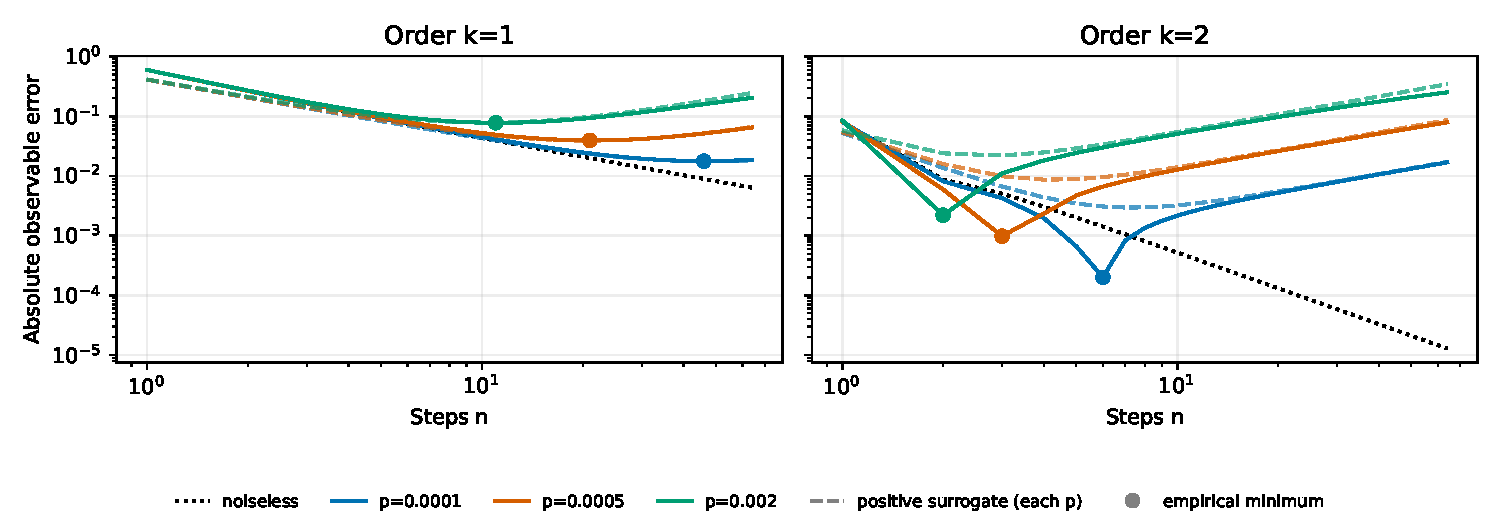
\includegraphics[width=\PlotWidth\textwidth]{error_curves.pdf}
\caption{Generated absolute errors for both orders. Solid colored curves are density-matrix results, dashed curves are the calibrated positive surrogate, and circles mark empirical minima. The dotted black curve is noiseless. Connecting the integer points is only a visual guide.}
\label{fig:error}
\end{figure}

The first-order curves exhibit a broad hardware-limited optimum, and the predicted depth is useful as a scale estimate. It is not exact: the asymptotic coefficient calibrated at large depth need not describe shallow formula errors, and the noise response need not remain exactly linear. The positive surrogate can understate or overstate the actual error; its fitted status supplies no universal bound.

For the symmetric formula, the much sharper dips are not evidence that the algorithmic approximation has suddenly acquired a higher asymptotic order. They arise because the positive noiseless bias can offset the negative noise-induced shift. Their location depends on the chosen observable and state. A narrow dip in one expectation does not certify closeness of the evolved density matrix to the ideal density matrix. The next section makes this sign issue explicit without changing the performance metric.

\section{Numerical observation: why error signs matter}
There is an exact identity at every depth:
\begin{equation}\label{eq:decompose}
 \mu_{n,p}-\mu_*=
 \underbrace{\mu_{n,0}-\mu_*}_{\text{algorithmic signed bias}}+
 \underbrace{\mu_{n,p}-\mu_{n,0}}_{\text{noise-induced signed shift}}.
\end{equation}
The metric is the absolute value of the left side. Adding the magnitudes of the terms on the right gives an upper bound if those \emph{actual} magnitudes are known; replacing them with calibrated asymptotic expressions need not preserve the bound.

\begin{figure}[ht]
\centering
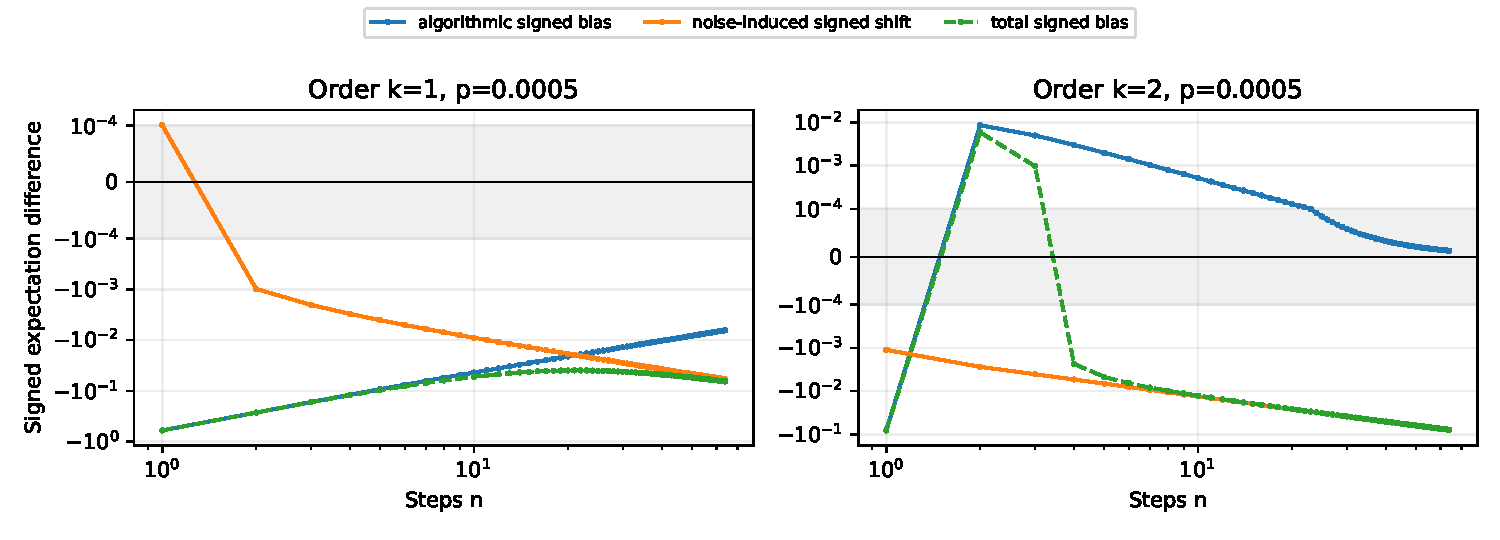
\includegraphics[width=\PlotWidth\textwidth]{signed_bias.pdf}
\caption{Generated decomposition of the observable bias at the middle noise rate. First-order errors reinforce over the useful depth range. Second-order errors can cancel. Separate symmetric-logarithmic vertical axes resolve the small second-order cancellation region while retaining the shallow-depth outlier. Gray shading marks the central linear band; bends at its edges reflect the axis scale, not a physical transition. These are signed components of the same absolute-error metric, not different objectives.}
\label{fig:signed}
\end{figure}

When the two biases have the same sign and magnitudes approximately $A/n^k$ and $Bn$, minimizing their sum is sensible. This accounts for the qualitative success of the first-order model in the example. When their signs differ, the leading approximation to the actual error is instead
\[
 e(n,p)\approx\abs{A/n^k-Bn}.
\]
Cancellation occurs at $n_{\rm cancel}=(A/B)^{1/(k+1)}$. In contrast, the positive surrogate is minimized at $n_*=(kA/B)^{1/(k+1)}$. Their ratio is $n_*/n_{\rm cancel}=k^{1/(k+1)}$, hence $2^{1/3}$ for $k=2$. The integer cancellation diagnostic agrees with $\CancelMatches$ of the $\CancelCases$ second-order grid optima in Table~\ref{tab:opt}. This is a post-hoc agreement on one observable, not a validated predictor. These expressions distinguish a cancellation dip from an envelope optimum. At shallow depths higher-order terms invalidate both simple expressions; the generated curves retain those points rather than selecting only a favorable asymptotic window.

The second-order formula also has more noise locations under the specified implementation. Consequently a smaller noiseless error does not automatically imply a smaller noisy error at a fixed depth. Comparing orders fairly requires specifying the compiler, gate support, and noise convention, not merely stating formal convergence orders.

There are two different limitations on the analytic prediction. One is \emph{calibration error}: a fitted $A$ or $c$ can fail outside its calibration region. The other is \emph{objective mismatch}: even perfectly known positive envelopes need not identify the minimum of a signed observable deviation. More accurate commutator constants address the former bound looseness but do not eliminate cancellation. The tutorial keeps these limitations separate rather than interpreting all discrepancies as statistical scatter; the curves in this figure contain no shot noise at all.

\section{Numerical observation: the stopping rule can be early or late}
Pauli outcomes are binomial with success probability $(1+\mu_{n,p})/2$. Independent samples at each depth are scanned using \eqref{eq:stop}. Pre-generating all depths is distributionally equivalent to sequential sampling until stopping.

There are $M=\Comparisons$ planned comparisons, $\delta=\DeltaVal$, and $\Reps$ repetitions per circuit/noise/shot-count case. The base seed is $\Seed$, with deterministic distinct offsets per case. The shot budgets $\ShotsLow$, $\ShotsMid$, and $\ShotsHigh$ give thresholds $\TauLow$, $\TauMid$, and $\TauHigh$ respectively. The largest budget is deliberately unrealistic: it reveals late stopping under resolvable noise drift. Binomial sampling avoids looping over individual shots.

\begin{table}[ht]
\centering\small
\begin{tabular}{ccrrrrrr}
\toprule
$k$ & $p$ & $S$ & Median & $e(\mathrm{stop})/e_{\min}$ & Early (\%) & Late (\%) & Cap (\%)\\
\midrule
1 & $0.0001$ & $1\times 10^{4}$ & 3 & 9.33 & 100.0 & 0.0 & 0.0 \\ 
1 & $0.0001$ & $1\times 10^{6}$ & 9 & 2.83 & 100.0 & 0.0 & 0.0 \\ 
1 & $0.0001$ & $1\times 10^{10}$ & 41 & 1.01 & 100.0 & 0.0 & 0.0 \\ 
1 & $0.0005$ & $1\times 10^{4}$ & 3 & 4.24 & 100.0 & 0.0 & 0.0 \\ 
1 & $0.0005$ & $1\times 10^{6}$ & 8 & 1.58 & 100.0 & 0.0 & 0.0 \\ 
1 & $0.0005$ & $1\times 10^{10}$ & 21 & 1.00 & 1.0 & 0.0 & 0.0 \\ 
1 & $0.002$ & $1\times 10^{4}$ & 3 & 2.23 & 100.0 & 0.0 & 0.0 \\ 
1 & $0.002$ & $1\times 10^{6}$ & 7 & 1.12 & 100.0 & 0.0 & 0.0 \\ 
1 & $0.002$ & $1\times 10^{10}$ & 64 & 2.62 & 0.0 & 100.0 & 100.0 \\ 
2 & $0.0001$ & $1\times 10^{4}$ & 2 & 40.68 & 100.0 & 0.0 & 0.0 \\ 
2 & $0.0001$ & $1\times 10^{6}$ & 2 & 40.68 & 100.0 & 0.0 & 0.0 \\ 
2 & $0.0001$ & $1\times 10^{10}$ & 64 & 84.28 & 0.0 & 100.0 & 100.0 \\ 
2 & $0.0005$ & $1\times 10^{4}$ & 2 & 6.07 & 100.0 & 0.0 & 0.0 \\ 
2 & $0.0005$ & $1\times 10^{6}$ & 2 & 6.07 & 73.0 & 0.0 & 0.0 \\ 
2 & $0.0005$ & $1\times 10^{10}$ & 64 & 80.64 & 0.0 & 100.0 & 100.0 \\ 
2 & $0.002$ & $1\times 10^{4}$ & 2 & 1.00 & 1.8 & 0.0 & 0.0 \\ 
2 & $0.002$ & $1\times 10^{6}$ & 5 & 11.04 & 0.0 & 100.0 & 0.0 \\ 
2 & $0.002$ & $1\times 10^{10}$ & 64 & 114.01 & 0.0 & 100.0 & 100.0 \\ 
\bottomrule
\end{tabular}

\caption{Generated Monte Carlo stopping results. Early and late compare the returned depth with $n_{\rm emp}$ in Table~\ref{tab:opt}. Their percentages exclude exact matches. The error ratio evaluates the exact error at the median stopping depth, divided by $e_{\min}=e(n_{\rm emp})$; it is not the median of per-run error ratios. ``Cap'' means no earlier pair triggered; it is a subset of late outcomes in this experiment, not an additional disjoint category.}
\label{tab:stop}
\end{table}

\begin{figure}[ht]
\centering
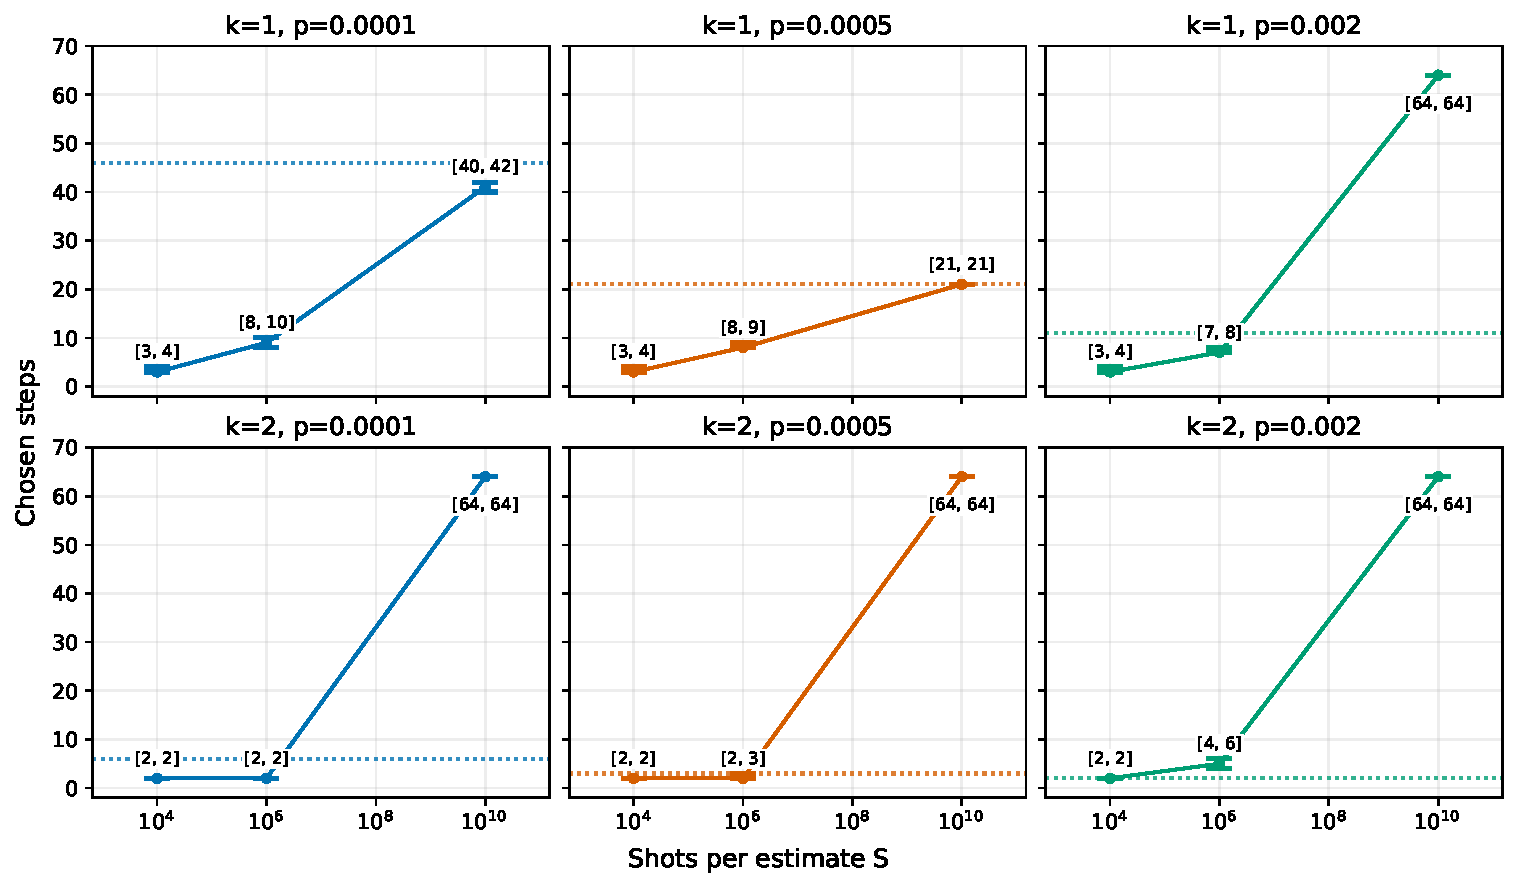
\includegraphics[width=\PlotWidth\textwidth]{stopping.pdf}
\caption{Generated stopping depths: medians with empirical \LowerPercentile--\UpperPercentile\ percentile ranges, not confidence intervals for the median. Each noise/order case has its own panel; capped error bars and bracketed endpoint labels show even zero-width or very narrow ranges without implying nonzero uncertainty. Horizontal dotted lines show each case's true finite-grid optimum. Values at $\Nmax$ are capped runs, not converged optima. More shots do not guarantee a better chosen depth.}
\label{fig:stop}
\end{figure}

Low budgets usually cause early stopping. At the highest budget, median stopping is late in $\LateHighCases$ of $\HighCases$ cases, not all cases: $k=1$, $p=\PLow$ is still early (depth $\EarlyHighDepth$ versus optimum $\EarlyHighOpt$), and the middle-rate first-order case matches its optimum. Very high budgets can expose late stopping under resolvable drift. This does not contradict the confidence theorem, which controls estimation error, not closeness to $\mu_*$. The seeded Monte Carlo percentages are observations, not probability guarantees.

\section{Limits, reproducibility, and responsible interpretation}
\paragraph{Bounds versus useful predictions.}
Commutator-based constants are principled but may be loose. Here the first-order block commutator norm is $\BlockComm$, giving $A_{\rm bd}=\ABound$ versus fitted $A=\AOne$ (a factor $\ALooseness$), while $2G=\NoiseBound$ versus fitted $c=\COne$ (a factor $\CLooseness$). The generated comparison below uses the continuous rigorous-bound optimum $\sqrt{A_{\rm bd}/(2Gp)}$:
\begin{center}
\begin{tabular}{crr}
\toprule
$p$ & Rigorous-bound $n_*$ & $n_{\rm emp}$\\
\midrule
$0.0001$ & 54.67 & 46 \\ 
$0.0005$ & 24.45 & 21 \\ 
$0.002$ & 12.22 & 11 \\ 
\bottomrule
\end{tabular}

\end{center}
The two looseness factors partly cancel in the optimum, but that numerical coincidence is not a guarantee. A minimum of a loose upper bound can be far from a minimum of the actual observable error. The fitted coefficients used in the numerical comparison are more descriptive, but they require calibration and provide no certificate. The exhaustive grid is intentionally small enough to reproduce; no global optimization claim is made beyond that grid.

\paragraph{Hardware realism.}
Uniform, independent gate-support depolarization omits coherent overrotations, leakage, crosstalk, temporally correlated noise, idle errors, and readout bias. Physical rotations can have duration-dependent errors, making $p$ depend on step size. Compiling a two-qubit rotation into several native gates changes the relevant channel and gate count. In such settings neither linear accumulation nor a single noise coefficient is automatic. The generalized exponent $\alpha$ is an algebraic extension, not a fitted physical noise law in this experiment.

\paragraph{Measurement and mitigation.}
Readout calibration drift can defeat the independent-shot model. Error mitigation may reduce bias while increasing estimator variance, and quasi-probability estimators need not remain in the interval assumed by the Hoeffding calculation. Their actual range or a suitable alternative concentration bound must be used. A task involving many observables requires an additional simultaneous-error allocation. Reporting an unresolved adjacent change should never be presented as a certificate of state fidelity.

\paragraph{What is reproduced.}
Run \texttt{python3\ run\_all.py} from the accompanying \texttt{code} directory. The script regenerates all figures, tables, numerical macros, bibliography metadata, and machine-readable results. Assertions check the symbolic minimum, nonconservation, a nonnegligible Trotter error, dense layer and channel cross-checks, Choi positivity, interior minima, and deterministic fixed-seed sampling. The manuscript is then compiled with \texttt{pdflatex} twice. Repeated seeded runs on the same numerical stack reproduce the samples exactly; floating-point details or random-library changes across versions can alter last digits or sample streams. Package versions are recorded in the generated results file.

\paragraph{Scope of the formal check.}
The accompanying Lean 4 + Mathlib check verifies the auxiliary polynomial inequality
and its scaled form, global minimality and the value at a positive stationary point
for $\alpha=1$ and positive natural-number $k$, and the arithmetic implication
$S\geq4\log(2M/\delta)/u^2\Rightarrow2M\exp(-Su^2/4)\leq\delta$.
Only standard Lean axioms are used. This does not formalize the general real-exponent
$\alpha$ theorem, uniqueness or existence of the stationary point, the operator or
channel bounds, the simulator, or the stopping heuristic. Hoeffding's inequality
itself is cited, not formalised, and neither the probability union bound nor the
sampling assumptions are machine-checked. The gate checks the local source against
the installed Mathlib library; it does not rebuild Mathlib.

\paragraph{Takeaway.}
A depth obtained by balancing a decreasing approximation term and an increasing noise term is a useful starting scale. It becomes a credible prediction only after checking the noise implementation, coefficient calibration, and observable-error signs. Finite-shot resolution supplies a defensible way to describe uncertainty in adjacent changes, but a stopping decision based on that resolution is still a heuristic. The explicit early and late failures are part of the lesson, not exceptions to hide.

\paragraph{Data and code availability.}
Code accompanies this manuscript and is available at
\RepoURL. Generated numerical data are included with the code.

\paragraph{Use of generative AI.}
The large-language-model assistants \AIAstra\ and \AIOpus, accessed through \AIPlatform, were used in the preparation of this tutorial, including code, computation, literature search, drafting, review and formalization. The author is responsible for the content, interpretation, references, and any remaining errors.

\begingroup\small
\begin{thebibliography}{9}
\bibitem{knee} George C. Knee, William J. Munro, \emph{Optimal Trotterization in universal quantum simulators under faulty control}, Physical Review A \textbf{91} (5) (2015), 052327. \href{https://doi.org/10.1103/physreva.91.052327}{doi:10.1103/physreva.91.052327}.
\bibitem{childs} Andrew M. Childs, Yuan Su, Minh C. Tran, Nathan Wiebe, Shuchen Zhu, \emph{Theory of Trotter Error with Commutator Scaling}, Physical Review X \textbf{11} (1) (2021), 011020. \href{https://doi.org/10.1103/physrevx.11.011020}{doi:10.1103/physrevx.11.011020}.
\bibitem{suzuki} Masuo Suzuki, \emph{General theory of fractal path integrals with applications to many-body theories and statistical physics}, Journal of Mathematical Physics \textbf{32} (2) (1991), 400-407. \href{https://doi.org/10.1063/1.529425}{doi:10.1063/1.529425}.
\bibitem{lloyd} Seth Lloyd, \emph{Universal Quantum Simulators}, Science \textbf{273} (5278) (1996), 1073-1078. \href{https://doi.org/10.1126/science.273.5278.1073}{doi:10.1126/science.273.5278.1073}.
\bibitem{hoeffding} Wassily Hoeffding, \emph{Probability Inequalities for Sums of Bounded Random Variables}, Journal of the American Statistical Association \textbf{58} (301) (1963), 13-30. \href{https://doi.org/10.1080/01621459.1963.10500830}{doi:10.1080/01621459.1963.10500830}.
\end{thebibliography}

\endgroup
\end{document}
